\section{Path Integral quantization of non-Abelian gauge theories}

\subsection{Photon/Abelian case refesher}
We had:
\begin{equation}
    S = -\frac{1}{4}\int F^2
\end{equation}
where the generating functional was:
\begin{equation}
    Z = \int \mathcal{D}A_\mu e^{iS[A]} = \int \mathcal{D} A_\mu \int \mathcal{D}\lambda \delta(g(A^\lambda))\det\frac{\delta g(A^\lambda)}{\lambda} e^{iS[A^\lambda]}
\end{equation}
with $A^\lambda_\mu = A_\mu - \p_\mu \lambda$. For example $g(A) = \p_\mu A^\mu(x) - \omega(x)$. In the above step, all that we use is a sort of completeness relation to introduce 1. We then see that the integrand can be made independent of $\lambda$, so:
\begin{equation}
    \begin{split}
        Z &= \left(\int \mathcal{D} \lambda\right)\int \mathcal{D}A_\mu \delta(\p_\mu A^\mu - \omega)\det \frac{\delta g(A^\mu)}{\lambda}e^{iS[A]}
        \\ &= \int \mathcal{D}A_\mu \delta(\p_\mu A^\mu - \omega)\det \frac{\delta g(A^\mu)}{\lambda}e^{iS[A]}
        \\ &\propto \mathcal{D}\omega e^{-i\int \frac{\omega^2}{2\xi}}
    \end{split}
\end{equation}
Thus:
\begin{equation}
    Z = \int \mathcal{D}A_\mu e^{iS'[A]}\det\frac{\delta g(A^\lambda)}{\lambda}
\end{equation}
With:
\begin{equation}
    S'[A] = -\int \frac{1}{4}F^2 + \frac{1}{2\xi}(\p_\mu A^\mu)^2
\end{equation}
\begin{equation}
    \frac{\delta g(\lambda)}{\lambda(y)} = \frac{\delta}{\delta \lambda(y)}\left(\p_\mu A^\mu(x) - \p^2\lambda(x)\right) = -\p^2\delta^4(x-y) \implies \det \frac{\delta g(\lambda)}{\lambda(y)} =  \det(-\p^2\delta^4(x-y))
\end{equation}
which is independent of $\lambda$, as it should be.

\subsection{Path integral for $U(N)$ gauge field}
We apply the same strategy to our $N^2$ $U(N)$ gauge fields $A_\mu^a$, $a = 1, \ldots, N^2$. We gauge fix each one; $g^a(A) = \p^\mu A_\mu^a - \omega^a$.

Then (introducing an integral of $1$ $N^2$ times):
\begin{equation}
    Z = \int \mathcal{D}A_\mu^a e^{iS[A]} = \int \mathcal{A}_\mu^a \int \mathcal{D}\lambda^a \prod_{b=1}^{N^2}\delta(g^b(A^\lambda))\det\frac{\delta g^b(A^\lambda)}{\lambda} e^{iS[A^\lambda]}
\end{equation}
Again the integral $\int \mathcal{D}\lambda^a$ evaluates to 1, so:
\begin{equation}
    Z = \int \mathcal{D}A_\mu^a\prod_{b=1}^{N^2}\delta(g^b(A^\lambda))\det\frac{\delta g^b(A^\lambda)}{\lambda} e^{iS[A^\lambda]} = \int \mathcal{D}\omega e^{-i\int \frac{1}{2\xi}\Tr(\omega^2)}
\end{equation}
with $\omega \equiv \omega^a T_a$. ThusL
\begin{equation}
    Z = \int DA_\mu^a e^{iS'[A]}\det\frac{\delta g^a(A^\lambda)}{\lambda^b}
\end{equation}
with:
\begin{equation}
    S'[A] = -\int \frac{1}{4}\Tr(F^2) + \frac{1}{2\xi}\Tr((\p_\mu A^\mu)^2).
\end{equation}
The determinant piece is now more interesting. Let us expand out the gauge transformed $A$:
\begin{equation}
    A_\mu^\lambda = e^{i\lambda}(A_\mu - o\p_\mu)e^{-i\lambda} \approx A_\mu - \p_\mu \lambda + i[\lambda, A_\mu]
\end{equation}
or:
\begin{equation}
    A_\mu^{\lambda\sp a} = A_\mu^a - \p_\mu \lambda^a - f_{bc}^{\sp\sp a} \lambda^b A_\mu^c
\end{equation}
The last term is what is new, and it will cause all the trouble. Computing the functional derivative:
\begin{equation}
    \frac{\delta g^a(x)}{\lambda^b(y)} = \frac{\delta}{\delta \lambda^b(y)}\left(-\p^\mu[(\p_\mu\delta_b^a + f_{bc}^{\sp\sp a}A_\mu^{\sp c})\lambda^b(x)]\right) = -\p^\mu\left[(\p_\mu \delta^a_b + f_{bc}^{\sp\sp a}A_\mu^{\sp c})\delta^4(x-y)\right]
\end{equation}
we see that this depends on $A$, in contrast to the Abelian case! So then:
\begin{equation}
    Z = \int \mathcal{D}A_\mu^a \det\left(-\p^\mu\left[(\p_\mu \delta^a_b + f_{bc}^{\sp\sp a}A_\mu^c)\delta^4(x-y)\right]\right)e^{iS'_{YM}[A]}
\end{equation}
What can produce a determinant from an integral? Let us recall that:
\begin{equation}
    \int d\v{x}e^{-\frac{1}{2}x^T M x} = \frac{C}{\sqrt{\det M}}
\end{equation}
Getting rid of the square root is easy; we can just do the same integral twice, or we can do an integral over complex numbers:
\begin{equation}
    \int d\v{z}e^{-z^\dag M z} = \frac{C}{\det M}.
\end{equation}
For Grassman variables (where we can just Taylor expand to first order because they square to zero):
\begin{equation}
    \int d\gv{\eta} e^{-\frac{1}{2}\gv{\eta}^T M \gv{\eta}} = C\sqrt{\det M}
\end{equation}
or with complex grassman variables:
\begin{equation}
    \int d\gv{\eta} d\bar{\gv{\eta}} e^{-\bar{\gv{\eta}}M \gv{\eta}} = C\det M
\end{equation}
so we can get determinants, and this is just a nice, Gaussian action! So, let's apply this trick; it will introduce some funny fermions into our path integral:
\begin{equation}
    \det(-\p^\mu(\p_\mu \delta^b_a + f_{bc}^{\sp\sp a}A_\mu)\delta^4(x-y)) \propto \int \mathcal{D}c \mathcal{D}\bar{c} e^{i\int \bar{c}_a\p^\mu(\p_\mu \delta^a_b + f_{bc}^{\sp\sp a}A_\mu^c)c_b}
\end{equation}
This introduces new fields! Specifically, it introduces $2N^2$ fermionic ``ghosts'' $c_{a=1, \ldots N^2}$ and $\bar{c}_a$.

So, our final result:
\begin{equation}
    Z = \int \mathcal{D}A \mathcal{D}c \mathcal{D}\bar{c} e^{iS_{YM}}
\end{equation}
with:
\begin{equation}
    S_{\text{YM, final}} = -\int \frac{1}{4}\Tr(F^2) + \frac{1}{2\xi}\Tr((\p_\mu A^\mu)) + \bar{c}_a\p^\mu \left([\p_\mu \delta^a_b + f_{bc}^{\sp\sp a} A_\mu^c]c_b\right)
\end{equation}

We get ghosts appearing in the diagrams which previously only contained gluons, as follows:

\begin{center}
    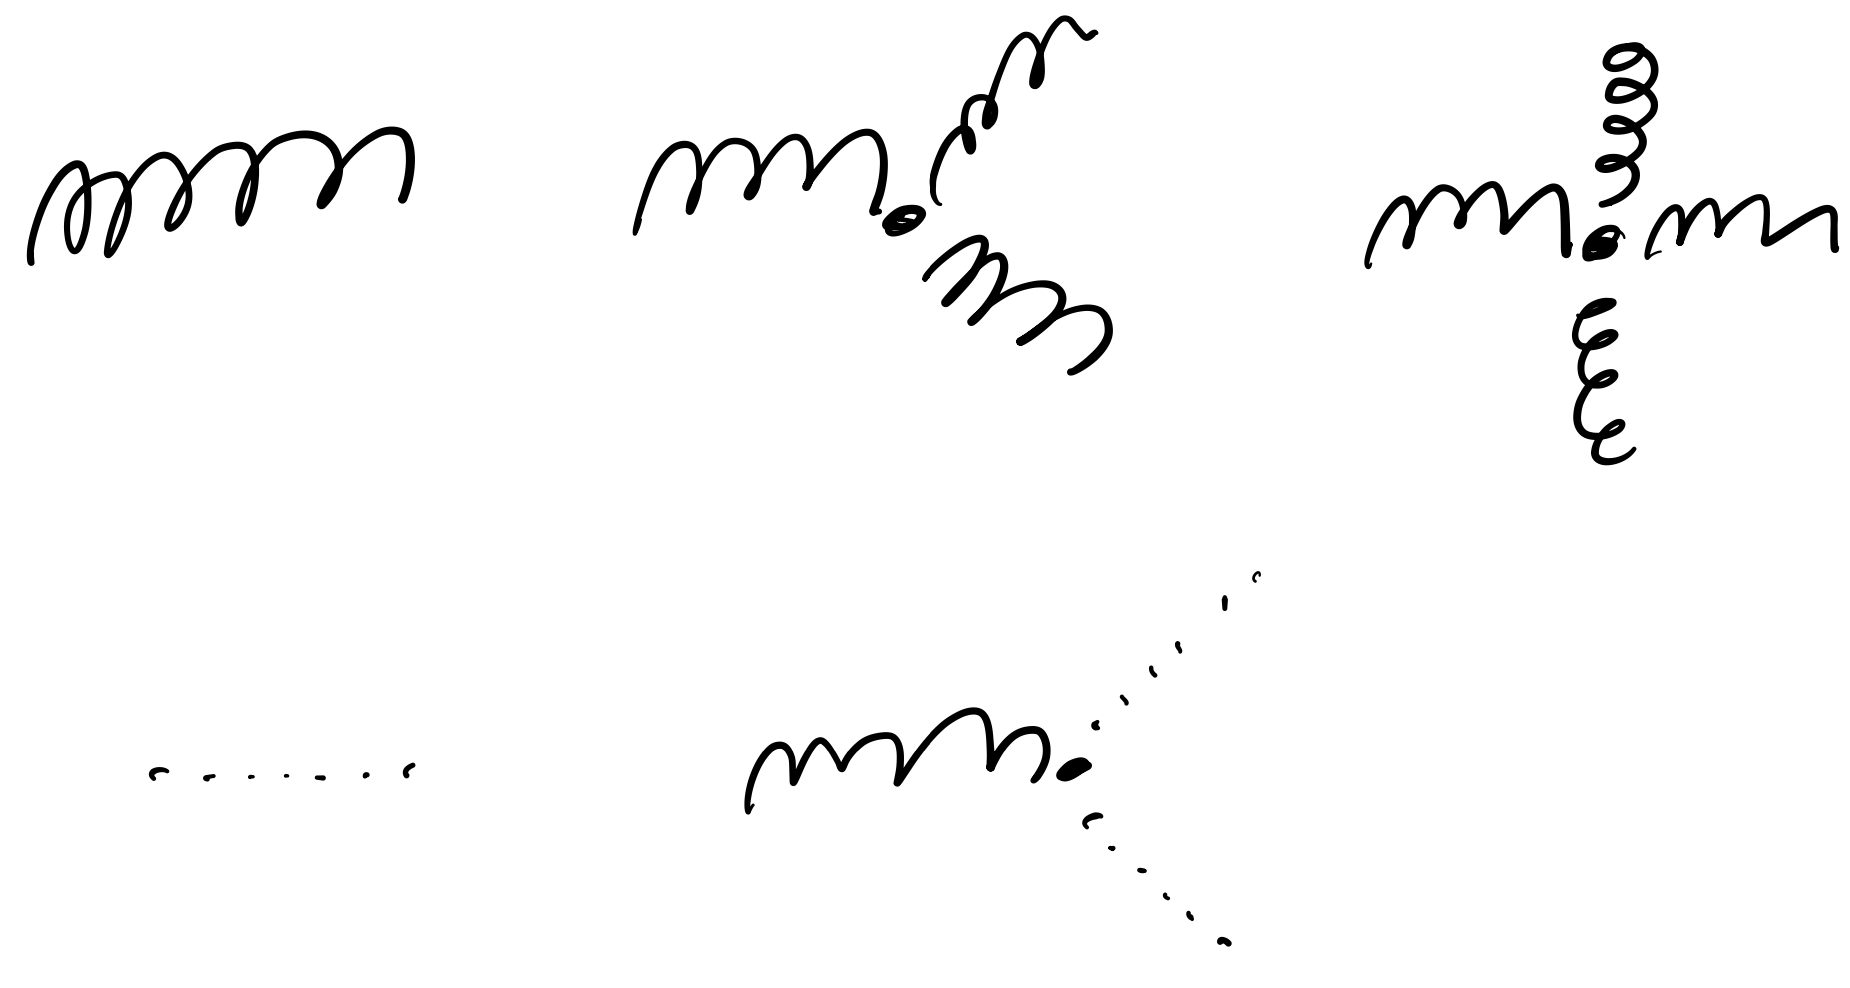
\includegraphics[scale=0.35]{Lectures/Images/lec17-gluonghosts.png}
\end{center}

Wwe could have very well done this for the Abelian case, but note that the structure factor $f_{bc}^{\sp\sp a} A_\mu^c$ vanishes in that case.

So - we have obtained our fully quantum description of QCD:
\begin{equation}
    Z = \int \mathcal{D}A\mathcal{D}\bar{\psi}\mathcal{D}\psi \mathcal{D}\bar{c}\mathcal{D}c e^{iS_{\text{QCD, final}}}
\end{equation}
with:
\begin{equation}
    S_{\text{QCD, final}} = \int \bar{\psi}(i\slashed{D} - m)\psi + S_{\text{YM, final}}
\end{equation}
one can look at the $\beta$ function for this theory - interestingly, depending on what $N$ is and how many fermions we have, we can change the sign of the $\beta$ function. So there is a rich landscape of non-Abeliean gauge theories, leading to lots of interesting phenomena. For example in QCD one finds that the $\beta$ function is the opposite of QED; the theory is UV-complete; it can predict everything microscopically, but at low energies it becomes strongly coupled and it is difficult to study quantitatively. Thus, it is a topic of current research to find techniques for QCD beyond perturbation theory.

\subsection{Wilson Lines}
We've figured out how to build gauge-invariant actions. We have local terms $\bar{\psi}(x)\psi(x)$. How do we come up with gauge-invariant terms for, e.g., quarks that are spatially separated? We do know how to create semi-local gauge invariant operators via using covariant derivatives, such as $\bar{\psi}D_\mu \psi$ and $\bar{\psi}D_\mu D_\nu \psi$.

Let's try to build a field $\tilde{\psi}_{x_2}(x_2)$ that transforms like $\psi(x_1)$. Currently, we have $\psi(x_2) \to U(x_1)\psi(x_2)$ which is not what we want, we want $\tilde{\psi}_{x_1}(x_2) \to U(x_1)\tilde{\psi}_{x_1}(x_2)$.

\begin{center}
    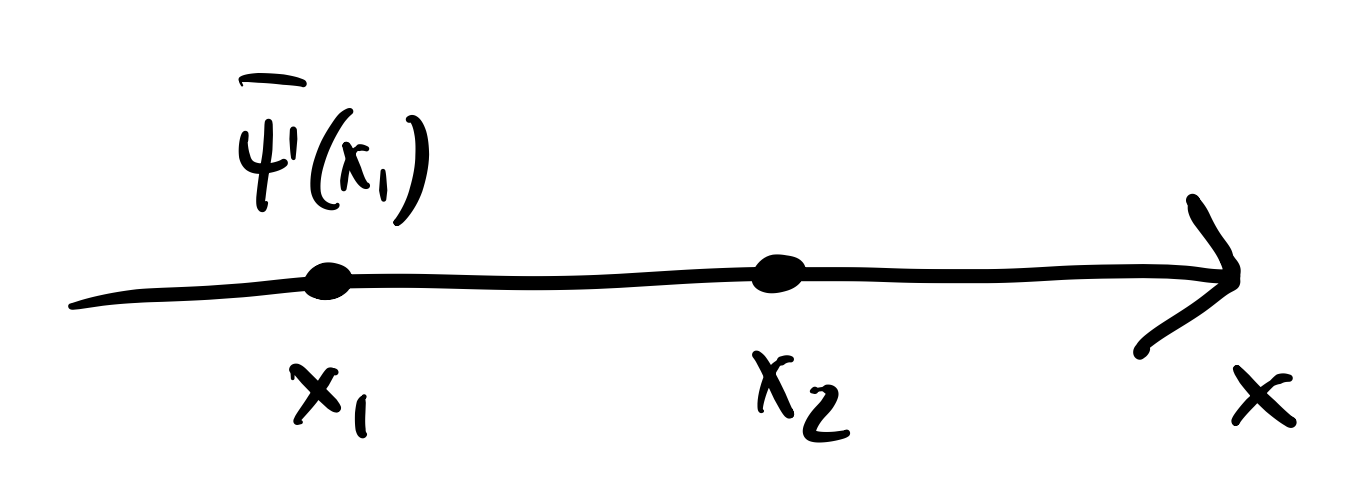
\includegraphics[scale=0.35]{Lectures/Images/lec17-nonlocalop.png}
\end{center}

Let's Taylor expand $\psi(x_2)$ around $x_1$:
\begin{equation}
    \psi(x_2) = \sum_{n \geq 0}\frac{(x_2 - x_1)^n}{n!}\p^n_{x_1}\psi(x_2)
\end{equation}
which transforms like $U(x_2)\psi(x_2)$, again not what we want. Let's now replace the derivatives above with covariant derivatives $D_x = \p_x + iA_x$:
\begin{equation}
    \tilde{\psi}_{x_1}(x_2) = \sum_{n \geq 0}\frac{(x_2 - x_1)^n}{n!}D_{x_1}^n\psi(x_1)
\end{equation}
This transforms like $U(x_1)\tilde{\psi}_{x_1}(x_2)$ as desired. This is because:
\begin{equation}
    D_x^a\psi(x_1) \to U(x_1)D_x^a\psi(x_1).
\end{equation}

We can now construct a gauge-invariant non-local/extended operator:
\begin{equation}
    \bar{\psi}(x_1)\tilde{\psi}_{x_1}(x_2) \to \tilde{\psi}(x_1)U^{-1}(x_1)U(x_1)\tilde{\psi}_{x_1}(x_2)
\end{equation}
Let's try to get a nicer expression for $\tilde{\psi}_{x_1}(x_2)$. Consider:
\begin{equation}
    \begin{split}
        \p_{x_1}\tilde{\psi}_{x_1}(x_2) &= \sum_{n \geq 0}\frac{(x_2 - x_1)^n}{n!}\p_{x_1}D^n_{x_1}\psi(x_1) - \sum_{n \geq 1} \frac{(x_2 - x_1)^{n-1}}{(n-1)!}D_{x_1}D_{x_1}^{n-1}\psi(x_1)
        \\ &= \sum_{n \geq 0}\frac{(x_2 - x_1)^n}{n!}(\p_{x_1} - D_{x_1})D_{x_1^n}\psi(x_1)
        \\ &= \sum_{n \geq 0}\frac{(x_2 - x_1)^n}{n!}(-iA_{x}(x_1))D_{x_1^n}\psi(x_1)
        \\ &= -iA_x(x_1)\tilde{\psi}_{x_1}(x_2)
    \end{split}
\end{equation}
so the operators obey a very simple evolution equation. This is fairly analogous to the time-dependent Schrodinger equation:
\begin{equation}
    \p_t \psi(t) = iH(t)\psi(t)
\end{equation}
whose solution is the time-ordered exponential:
\begin{equation}
    \psi(t_1) = \mathcal{T}e^{-i\int_{t_2}^{t_1}H(t')dt'}\psi(t_2)
\end{equation}
So for us, the solution is just the path-ordered exponential:
\begin{equation}
    \tilde{\psi}_{x_1}(x_2) = \mathcal{P}e^{-i\int_{x_2}^{x_1}dx'A_x(x')}\tilde{\psi}_{x_2}(x_2)
\end{equation}
but, $\tilde{\psi}_{x_2}(x_2) = \psi(x_2)$ (from the definition, we can see that all but the $n = 0$ term vanishes). So, our gauge-invariant object is:
\begin{equation}
    \bar{\psi}(x_1)\tilde{\psi}_{x_1}(x_2) = \bar{\psi}(x_1)\mathcal{P}e^{-i\int_{x_2}^{x_1}dx A_x(x)}\psi(x_2)
\end{equation}
where we define the Wilson-line operator:
\begin{equation}
    W_{x_1, x_2} \equiv \mathcal{P}e^{-i\int_{x_2}^{x_1}dx A_x(x)}
\end{equation}

\begin{center}
    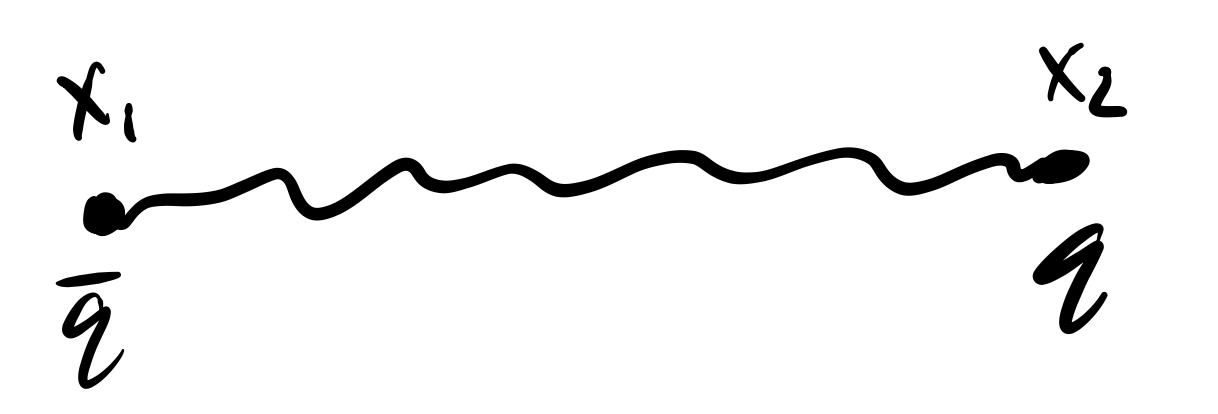
\includegraphics[scale=0.35]{Lectures/Images/lec17-wilsonline.png}
\end{center}

Since $ \bar{\psi}(x_1)\tilde{\psi}_{x_1}(x_2)$ is Gauge invariant, this tells us that the Wilson line operator transforms as:
\begin{equation}
    W_{x_1, x_2} \to U(x_1)W_{x_1, x_2}U^{-1}(x_2)
\end{equation}
We can generalize this construction to arbitrary paths:
\begin{equation}
    W_P = \mathcal{P}e^{-i\int_P dx^\mu A_\mu(x)} \to U(x_1)W_P U^{-1}(x_2)
\end{equation}

\begin{center}
    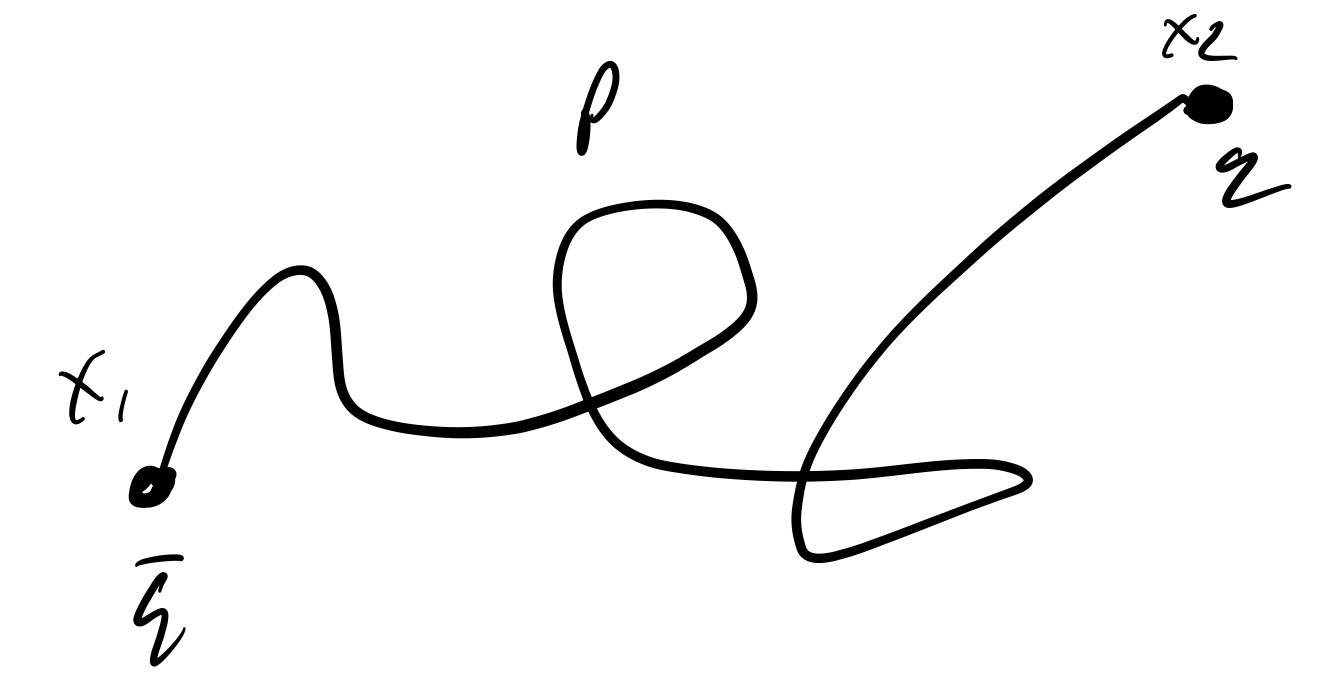
\includegraphics[scale=0.35]{Lectures/Images/lec17-wilsonlinepath.png}
\end{center}

We can also define this for a closed loop:
\begin{equation}
    W_C = \mathcal{P}e^{-i\oint_C dx^\mu A_\mu(x)} \to U(x)W_C U^{-1}(x)
\end{equation}
Where the Wilson-loop observables:
\begin{equation}
    W_C = \Tr(\mathcal{P}e^{-i\oint_C dx^\mu A_\mu})
\end{equation}
are gauge invariant!

\begin{center}
    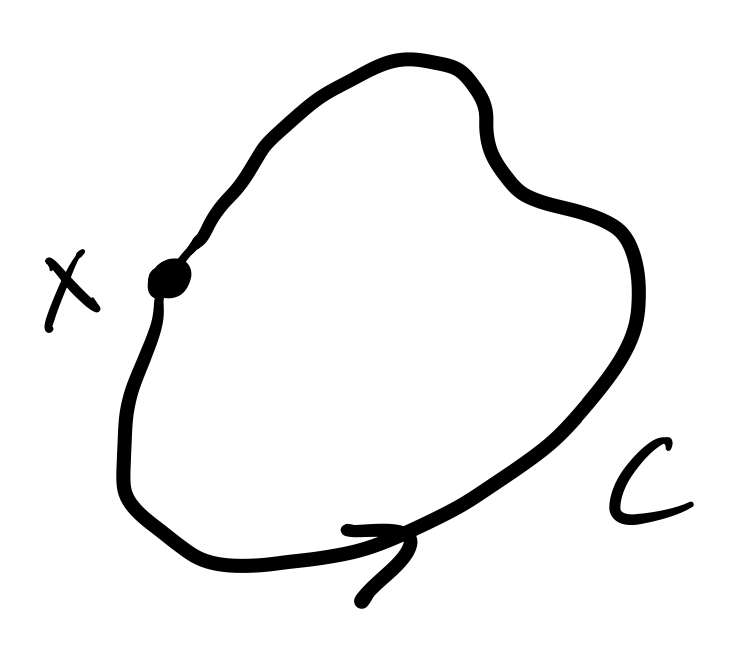
\includegraphics[scale=0.35]{Lectures/Images/lec17-wilsonloop.png}
\end{center}

A few comments:
\begin{itemize}
    \item For very small loops $C$, they reduce to gauge-invariant \emph{local} observables; using Stokes' theorem (this is done in Peskin 15.3):
    \item \begin{equation}
        W_C \sim 1 - i\Tr(F_{xy})\text{Area}(C) + \text{const.} \Tr(F_{xy}F_{xy})(\text{Area}(C))^2 + \ldots
    \end{equation}
    \item They can be used as order parameters; if we have $\avg{W_C} \sim e^{-\text{area}(C)}$ then we are in the confined phase (there is tension), and if $\avg{W_c} \sim e^{-\text{perimeter}(C)}$ then we are in the deconfined phase, without membrane tension. In modern language, we would associate this with the spontaneous breaking of higher-form symmetries.
    \item Wilson loops play a key role in topological phases/QFTs. They have the property that $\avg{W_CW_{C'}} \propto \text{linking}(C, C')$:
    \begin{center}
        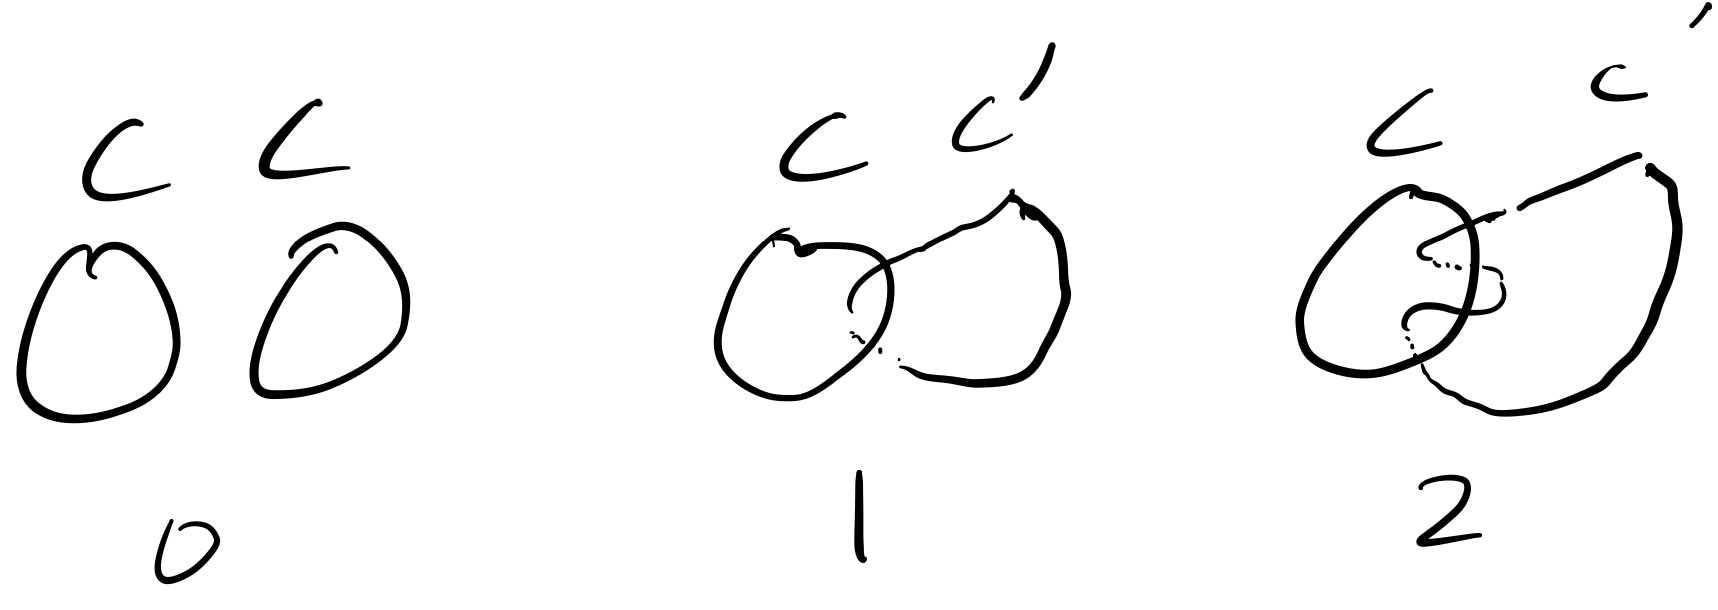
\includegraphics[scale=0.35]{Lectures/Images/lec17-linking.png}
    \end{center}
    
    And that $\avg{W_C} \propto \text{self-linking}(C)$:

    \begin{center}
        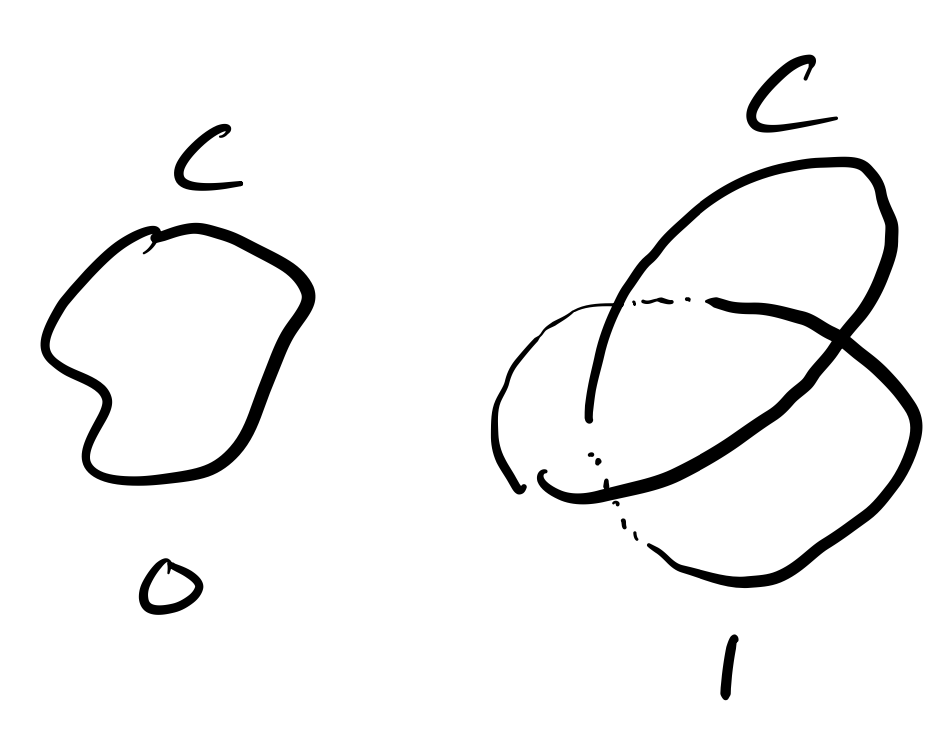
\includegraphics[scale=0.35]{Lectures/Images/lec17-selflinking.png}
    \end{center}

    They are very useful as probes in theories where the characteristics are non-local/local order parameters do not exist.
\end{itemize}

This is the end of QFT II - it's been a fun ride, and QFT has many many more beautiful aspects and topics. I hope you keep learning!